\chapter{PySPH: Design Philosophy}

In this chapter, an outline of the design of the PySPH \cite{prabhu_puri} tool is laid out. PySPH is an open-source, objected oriented Python based framework for SPH simulations with the performance critical portions implemented in Cython. The PySPH tool is flexible, user-friendly and allows for quick prototyping and extension to new problems.

\section{Abstractions for Numerical Implementation}

In order to motivate and explain the abstractions made for the numerical implementation, we consider a general SPH discretization (Equations \eqref{eq:Disc_SPH}) for the continuum equations for Mass, Momentum and Energy balance (Equations \eqref{eq:balance_laws}):

\begin{eqnarray} \label{eq:balance_laws}
\frac{D\rho}{Dt} &=& -\frac{1}{\rho} \nabla \cdot \vec{v} \nonumber \\
\frac{D{\vec{v}}}{Dt}&=&\vec{{\bf{k}}} + \frac{1}{\rho} \frac{\partial \tau^{lm}}{\partial x_m} \hat{l} \\
\frac{D{\it{e}}}{Dt}&=& -\frac{1}{\rho}\nabla \cdot \vec{q} + \frac{1}{\rho}\frac{\partial {\it{v}^{l}} }{\partial x_m}\tau^{lm} \nonumber
\end{eqnarray}

{\raggedright{where,}}\\
$\frac{D}{Dt}(\varphi) = $ Material Derivative of the field variable $\varphi = \left(\frac{\partial}{\partial t} + \vec{v}\cdot\nabla\right)(\varphi)$ \\
$\rho = $ Mass per unit volume in the limit that volume goes to zero at any point in the continuum\\
$\vec{v} = $ Velocity vector associated with a point particle\\
$\vec{{\bf{k}}} = $ Body Force per unit mass\\
$\tau^{lm} = $ Components of the stress tensor field\\
$e = $ Internal Energy per unit mass\\
$\vec{q} = $ Heat Flux Vector (heat energy transferred per unit time per unit area along the direction of heat flow) 

\newpage

\begin{eqnarray}\label{eq:Disc_SPH}
 \frac{D\rho_{a}}{Dt} &=& \sum_{b \in \Omega_{r}} m_{b}{\mathcal{D}}_{ab}(\vec{v})\cdot {\nabla}_{i} W_{ab}(h) \nonumber \\
 \frac{Dv^{i}_{a}}{Dt} &=& \sum_{b \in \Omega_{r}} m_{b}{\mathcal{F}}_{ab}(\rho ,P,\vec{v})\frac{\partial}{{\partial x}^{i}}W_{ab}(h)\\
 \frac{De_{a}}{Dt} &=& \sum_{b \in \Omega_{r}} m_{b}{\mathcal{E}}_{ab}(\rho ,P,\vec{v}) \cdot W_{ab}(h) \nonumber
\end{eqnarray}

{\raggedright{where,}}\\
${\rho}_a = $ Density of the particle ``a'' \\
$\Omega_{r} = $ Hypersphere of Influence of radius $\kappa$h\\
$m_b = $ mass of the particle ``b''\\ 
$v^{i}_{a} = i^{th}$ component of velocity of the particle ``a'' \\
$W_{ab} = $ Smoothing Kernel\\
$e_a = $ Internal Energy per unit mass of the particle ``a''\\

Referring to Figure \ref{fig:nearest_neighbors}, we see how the properties of a particle ``a'' evolves with via its interaction with nearest neighbours represented by particles ``b'' in the hypersphere $\Omega_{r}$; the descriptions of the terms $\kappa$ and ``h''  are given in section \ref{kappa}

\begin{figure}[htb!]
\centering
\setlength\fboxsep{0pt}
      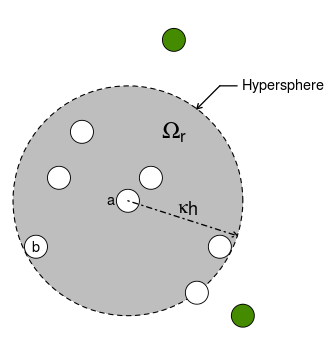
\includegraphics[scale=0.6]{figures/SpInfDiscrete_R.png} 
\caption{{\small{Neighbors List for a Particle ``a''}}}
\label{fig:nearest_neighbors}
\end{figure}

The terms $\mathcal{D}, \mathcal{F}$ and $\mathcal{E}$ are representations of the ``fluxes'' of mass, momentum and energy which contribute to the properties of particle ``a''. Based on the (non-exhaustive) discretizations given in Equations \eqref{eq:Disc_SPH}, PySPH incorporates the following abstractions:

\begin{itemize}
\item \textbf{\textit{Particle Container: }}It is the data structure which represents the arbitrary collections of particles inherent to the SPH method. The material species is represented as a collection of arrays (C++ vectors) describing the required properties. The default particle container comes with representations for the position, velocity, acceleration, pressure, mass, smoothing length and density along with a unique global index(gid), processor id(pid) and a tag\footnote[3]{\url{http://pysph.readthedocs.io/en/latest/reference/particle_array.html}}. Additional properties, if required by the problem can be easily added on the fly. 

\item \textbf{\textit{Nearest Neighbour Queries: }} As mentioned in Section \ref{kappa}, the keeping track of the nearest neighbours of any particle as specified by the hypersphere of influence(Figure \ref{fig:nearest_neighbors}) is computationally the most costly aspect of an SPH simulation. For performing such queries, Nearest Neighbour Particle Search (NNPS) Algorithms are used. By default PySPH implements a Linked List based NNPS; there are however a few more implementations to choose from\footnote[4]{\url{http://pysph.readthedocs.io/en/latest/reference/nnps.html}}.

\item \textbf{\textit{Interaction Physics: }}Based on the specific application area, the physics of the problem defines the nature of the general interaction terms  $\mathcal{D}, \mathcal{F}$ and $\mathcal{E}$ appearing in Equations \ref{eq:Disc_SPH}; there may also be inclusions of viscous stress and artificial viscosity terms for numerical stability of the scheme (more information of details for SPH in specific applications could be ~ found ~ at ~ (for example) ~ \cite{price}, ~ \cite{monaghan_ARFM}, \cite{monaghan_physics}, \\ \cite{volker_springel}).\\The Interaction Physics abstraction defines with these descriptions in the context of ``solving'' Equations \ref{eq:Disc_SPH} to obtain the accelerations of the particles.

\item \textbf{\textit{Integrator: }}Post completion of the particle interactions, the solution is updated in time using an Integrator\footnote[5]{\url{http://pysph.readthedocs.io/en/latest/reference/integrator.html}} step. These integrators can be include multiple-stages wherein intermediate storage of the properties is inherently available. 

\item \textbf{\textit{Miscellaneous: }}Lastly, data structures, routines and tools to construct solvers, equations, post process the results etc. are required. For post processing, the MayaVi\footnote[6]{\url{http://code.enthought.com/projects/mayavi/}} tool is utilized whereas all other requirements are addressed via routines in the source-code.
\end{itemize} 

\section{Design}


%
%By our first goal, we intend to build a model that on the basis of the histone modifications' data can predict for us the expression level of a gene in CD4$+$ T cells. More technically, we want this system to act as a {\em{classifier}} that is capable of predicting the gene expression levels in the concerned cells based only on these histone modifications as features. Details of this classification model are discussed ahead.
%
%
%\section{Classification Model}
%Intuitively, in brief, {\em{classification}} is the problem of identifying the class or the category of a new observation from an already known set of classes on the basis of data/observations that the classifier is trained on. This {\em{`training'}} data is a collection of observations whose class memberships are known in advance. For observations of a particular class, the classifier tries to note the values their characteristic features take or the pattern they follow, if any, and accordingly it later attempts to classify any new observations it comes across. This is very typically known as {\em{learning from data}}. A more mathematical explanation of classification is deferred to a later point in this thesis.
%
%For our work, from the histone modifications' data discussed, we have exactly 21 histone methylations' information as our features of each  observation input to the classifier. The corresponding gene expression level is the response variable for each input. But what we have overlooked about the gene expressions until now is that the gene expression levels are basically intensity values represented by their logarithms taken to base 2. In fact these intensities are the number of mRNA molecules that are produced from each gene whose logarithms are then computed. Hence these are inherently {\em{`continuous'}} values. With an aim to predict the expression level we have only talked about classes, which are always to be discrete. The next section describes in short how we obtained discrete classes from the continuous response variable.
%
%\section{Methodology}
%We collected about 26,000 instances, each with 21 features, and their corresponding expression levels. These features were the 21 methylations' counts falling in the promoter regions. The gene expression levels of these instances ranged approximately from 2.0 to just over 14.0 on the logarithmic scale. You may recollect from Figure~\ref{fig:barskiimgred} earlier that the negative correlation between a methylation and active genes was clearly visible. So we simply decided upon 2 optimal threshold values, one that marks the instances where the genes are active or highly expressed and the other marking repressed or inactive genes. The Figure~\ref{fig:distgene} depicts this via a frequency histogram of gene expression levels of all the 26,000 instances. It is worth to note here that a repressed gene does not necessarily mean an inactive gene.
%
%\begin{figure}[htb!]
%\centering
%\setlength\fboxsep{0pt}
%      \fbox{\includegraphics[width=4.6in, height=2.3in]{figures/gene-expr-dist}}
%\caption{{\small{Frequency histogram showing distribution of gene expression levels in CD4$+$ T cells}}}
%\label{fig:distgene}
%\end{figure}
%
%One heuristic to decide the lower threshold as 3.0 and upper threshold as 8.0 is that we also looked to have just enough number of instances for the classifier to learn the classes well. We thus formed a binary classification model \textendash \space class label `+1' if the expression level is beyond 8.0 and class label `$-$1' if under 2.0.
%
%\section{Results}
%Here we discuss and analyze the model performance and what measures were taken in terms of tuning the model parameters to maximize its performance.
%
%Since we have built a binary classification model here, what we mean by maximizing the model performance is that we would like the model to learn the intricacies of the problem at hand and be able to accurately discriminate between the two classes. Ideally, the classifier could correctly predict the class labels for each and every new observation it makes, giving an accuracy of 100\%. We employed a support vector classifier, also called a support vector machine (SVM)~\cite{tibshirani:stat, vapnik:maxmargin}. The details of the support vector classifier with the parameter values we used are given next.
%
%\subsection{Support Vector Classification}
%We used `LIBSVM - A Library for Support Vector Machines' created by Chih-Chung Chang and Chih-Jen Lin \cite{cjlin:libsvm} for implementing our classification model. A simple support vector classifier is a binary linear classifier which can perform a non-linear classification with what is popularly known as the kernel trick \cite{vapnik:maxmargin}. We worked with linear and polynomial kernels to start with. Though the dimension of our feature space was only 21, which isn't so high considering the typical dimensionality issues SVM is capable of handling otherwise, we still had a large number of example instances to train SVM on, about $26,000$ instances. This made it difficult for SVM employing linear and polynomial kernel to converge to optimal maximum margin hyperplanes within 100,000 iterations. We thus opted to work with a radial basis kernel. More on the kernel trick in appendix.
%
%Thus, the tuned set of values for all parameters for the classifier are given below:
%
%\begin{table}[htb!]
%\centering
%	      \begin{tabular}{|l | r|}
%	      \hline
%	      {\textbf{Parameter}} & {\textbf{Values}}\\
%	      \hline
%	      Cost & 10\\
%	      Gamma for radial basis kernel & $1$ x $10^{-5}$\\
%	      Folds for cross-validation & 10\\
%	      \hline
%	      \end{tabular}
%	      \caption{\small{Tuned parameter values for SVM}}
%        \label{tab:svmtunedvalues}
%\end{table}
%
%
%
%\subsection{Receiver Operating Characteristics Curve}
%
%Simply put, this curve measures the operating characteristics of a signal receiver. In other words it tells us the receiver's capability to accurately distinguish signal from noise. Receiver Operating Characteristics of a classifier shows its performance as a trade off between {\em{selectivity}} and {\em{sensitivity}}. It is a plot of {\em{`true positives'}} vs. the {\em{`true negatives'}}. In place of {\em{`true negatives'}}, one could also use {\em{`false positives'}} which are essentially \{1 - {\em{`true negatives'}}\}. This is plotted on a scale of 0-1 for both the axes. This curve always goes through (0,0) and (1,1).
%
%A classifier's performance can be evaluated by knowing its confusion matrix (appendix). We use that matrix to plot a ROC curve for a classifier and the area under the curve (AUC) of this plot pictorially tells us the classifier's accuracy \textendash \space the discriminative power of the classifier. The ROC curve of an ideal classifier (100\% accuracy) has an AUC of 1, with 0.0 {\em{`false positives'}} and 1.0 {\em{`true positives'}} (all new observations correctly classified). On the contrary, the ROC curve of what we call a `random guess classifier', when the classifier is completely confused and cannot at all distinguish between the two classes, has an AUC of 0.5, the {\em{`x $=$ y'}} line in the plot.
%
%Figure~\ref{fig:rocsimple} is such a ROC curve of binary classification with only the 21 histone modifications predicting gene expression levels. In this and all the following ROC curves we have also denoted the responses for (a) an ideal classifier in \textcolor{blue}{blue} and (b) the random guess classifier in {\textbf{\textcolor{turquoise}{turquoise blue}}}. 
%
%\begin{figure}[htb!]
%\centering
%\setlength\fboxsep{0pt}
%      \fbox{\includegraphics[width=3.5in, height=2.15in]{figures/roc-filled-light2}}
%\caption{{\small{ROC curve of binary classification with only histone modifications predicting gene expression levels}}}
%\label{fig:rocsimple}
%\end{figure}
%
%We used a window size of 3000 bp, relative to the TSS, as the promoter region, 2000 bp upstream and 1000 bp downstream. But this window size can really be anything, because we only know that the promoter region for a gene is a few base pairs long and lies in vicinity to that gene. Hence, we varied this window size with combinations of different upstream downstream sizes relative to the TSS. The bar-plot in Figure~\ref{fig:barplot} depicts the AUCs of the ROC curves obtained with these different combinations of upstream downstream window sizes \textendash \space upstream abbreviated as U and downstream as D.
%
%
%\begin{figure}[htb!]
%\centering
%\setlength\fboxsep{0pt}
%      \fbox{\includegraphics[width=3.5in, height=2.15in]{figures/bars}}
%\caption{{\small{Barplot of the AUCs for combinations of upstream/downstream window sizes}}}
%\label{fig:barplot}
%\end{figure}
%
%We observe that our classification model features have demonstrated a high discriminative ability with all the various window sizes. But why, we thought, should this be the case? Is our model so convincingly capable of discriminating the classes? To satisfy ourselves of our classifier, that it itself isn't doing something outright wrong insulated from the domain perspective, we attempted to confuse our classifier. For all the training instances fed to the classifier, we permuted their class labels with uniform randomness. So the feature set for the training data now may or may not exhibit the earlier structure/pattern since all instances with the same true class label have now got randomly dispersed in either of the classes. In such a scenario we expect the classifier to thus behave as a `random guess classifier'. Our ROC curve for this training data with randomized class labels is Figure~\ref{fig:rocrandom}. We have retained the upstream/downstream window sizes to 2000 and 1000 bp respectively.
%
%\begin{figure}[htb!]
%\centering
%\setlength\fboxsep{0pt}
%      \fbox{\includegraphics[width=3.5in, height=2.15in]{figures/randomized-plot}}
%\caption{{\small{ROC curve with randomized class labels}}}
%\label{fig:rocrandom}
%\end{figure}
%
%
%As the curve depicts, our classifier does get confused with the AUC falling to 0.4912. This corroborates our methodology. What remains to be checked is whether we can garner a similar support  for these accuracies from the domain perspective.
%
%We performed similar classification procedures in 2 more, different ways. Since we had collected these feature values from the promoter regions of the genes to predict the gene expression levels, as a first we moved out of the promoter region of these genes and performed the same procedure of collecting the modifications' values in 3000 bp long windows. More specifically, we moved away from the TSS by 100,000 bp and considered similar windows there to predict the expression levels of genes lying hereof. The ROC curve for these specifications are given in Figure~\ref{fig:rocaway}. The AUC has reduced comparatively; AUC = 0.7622 $<<$ 0.9727.
%
%\begin{figure}[htb!]
%\centering
%\setlength\fboxsep{0pt}
%      \fbox{\includegraphics[width=3.5in, height=2.15in]{figures/away-roc}}
%\caption{{\small{ROC curve after moving away by 100,000 bp from the promoter region}}}
%\label{fig:rocaway}
%\end{figure}
%
%As a second, we attempted to play with the way we have generated the two classes from our response variable. The earlier lower threshold was changed from 2.0 to a range of $4.0-5.0$. Thus, effectively, we diminished the distance between the two classes expecting to have made it at least little more difficult for the classifier to discriminate between the two class members now than the initial setting. The distance here being their separation on the {\em{x}}-axis, denoting the expression levels. Figure \ref{fig:distclass1} and \ref{fig:rocclass1} show the change in class boundaries and the corresponding ROC curves respectively.
%
%\begin{figure}[htb!]
%\centering
%\setlength\fboxsep{0pt}
%      \fbox{\includegraphics[width=4.6in, height=2.3in]{figures/gene-expr-dist2-4-5}}
%\caption{{\small{Distribution of gene expression levels in CD4$+$ T cells with a varied class boundary I}}}
%\label{fig:distclass1}
%\end{figure}
%
%\begin{figure}[htb!]
%\centering
%\setlength\fboxsep{0pt}
%      \fbox{\includegraphics[width=3.5in, height=2.15in]{figures/vary-4-5}}
%\caption{{\small{ROC curve for varied class boundary I}}}
%\label{fig:rocclass1}
%\end{figure}
%
%We moved the classes more closer to each other changing the lower class boundaries to $5.0-6.0$. Each time we made sure that the classifier also has enough examples to train on. The AUC now reduced to 0.8154 (Figure~\ref{fig:distclass2} and ~\ref{fig:rocclass2}). 
%
%
%\begin{figure}[htb!]
%\centering
%\setlength\fboxsep{0pt}
%      \fbox{\includegraphics[width=4.6in, height=2.3in]{figures/gene-expr-dist2-5-6}}
%\caption{{\small{Distribution of gene expression levels in CD4$+$ T cells with varied class boundary II}}}
%\label{fig:distclass2}
%\end{figure}
%
%\begin{figure}[htb!]
%\centering
%\setlength\fboxsep{0pt}
%      \fbox{\includegraphics[width=3.5in, height=2.15in]{figures/vary-5-6}}
%\caption{{\small{ROC curve for varied class boundary II}}}
%\label{fig:rocclass2}
%\end{figure}
%
%
%Thus we satisfied ourselves on both methodology and domain fronts. The histone modifications do seem to have a considerably high discriminative capability in terms of predicting whether the gene is highly expressed or not.
%
%\section{Goals revisited}
%Of our goals:
%    \begin{enumerate}
%     \item to predict expression level of a gene by histone modifications at its promoters; and
%     \item to characterize tissue specificity of promoters using these histone modifications,
%    \end{enumerate}
%the tissue specificity of promoters is still to be dealt with. The next chapter deals with this and explains what prompted us to believe in histone modifications, the epigenetic factors, to characterize such tissue specificity.
